\documentclass[a4paper,12pt]{article}
\usepackage[utf8]{inputenc}
\usepackage[english,russian]{babel}
\usepackage{amsmath}
\usepackage[dvipsnames]{xcolor}
\usepackage{geometry}
\usepackage{anyfontsize}
\usepackage{ragged2e}
\usepackage{array}
\usepackage{colortbl}
\usepackage{graphicx}
\usepackage{blindtext}
\usepackage{multicol}
\usepackage{tikz}

\setlength{\columnsep}{0.7cm}
\geometry{top=0cm, bottom=0cm, left=1.3cm, right=1.3cm}

\begin{document}
\thispagestyle{empty}

\noindent
\makebox[\textwidth][c]{
    \colorbox{Plum}{
        \parbox{\dimexpr\textwidth-2cm\relax}{
            \vspace{4.1em}
            \centering 
            \textcolor{white}{\Large\textbf{З А Д А Ч Н И К }}
            { }
            \textcolor{white}{\Large\textbf{ « К В А Н Т А »}}
            \vspace{0.4em}
        }
    }
}

\begin{center}
    \vspace{-0.3em}
    {\fontsize{28}{15}\selectfont
    \textcolor{Plum}{\textbf{З}}\textbf{адачи}} \\
    {\fontsize{28}{15}\selectfont
    \textbf{по математике и физике}}
    \vspace{-0.3em}
\end{center}

\small{\textbf{\textit{
    Этот раздел ведется у нас из номера в номер с момента основания журнала. Публикуемые
    в нем задачи нестандартны, но для их решения не требуется знаний, выходящих за рамки
    школьной программы. Наиболее трудные задачи отмечаются звездочкой. После формулировки 
    задачи мы обычно указываем, кто нам ее предложил. Разумеется, не все эти задачи 
    публикуются впервые.}}}

\small{\textbf{\textit{
    Решения задач по математике и физике из этого номера следует отправлять по электронным 
    адресам: math@kvant.ras.ru и phys@kvant.ras.ru соответственно или по почтовому адресу: 
    119296 Москва, Ленинский проспект, 64-А, «Квант».}}}

\small{\textbf{\textit{
    Условия каждой оригинальной задачи, предлагаемой для публикации, вместе с Вашим 
    решением этой задачи присылайте по тем же адресам.}}}

\small{\textbf{\textit{
    Задача М2479 предлагалась на XIII Олимпиаде имени И.Ф.Шарыгина, задача М2481 – на LVIII 
    Международной математической олимпиаде.}}}

\vspace{0.5em}
\normalsize

\begin{multicols}{2}

\justifying
\noindent
\textbf{Задачи М2478–М2481, Ф2485–Ф2488} \\[0.5em]
\textcolor{Plum}{\textbf{M2478.}}
Дана «таблица умножения» \textit{n} × \textit{n}
(т.е. таблица, в которой на пересечении строки с номером
\textit{k} и столбца с номером \textit{m} записно число \textit{km}
(на рисунке 1 показана
\vspace{-0.5em}
\begin{center}
    \renewcommand{\arraystretch}{1.4}
    \begin{tabular}{>{\centering\arraybackslash}p{0.4em}
                    >{\centering\arraybackslash}p{1.7em} 
                    >{\centering\arraybackslash}p{1.7em} 
                    >{\centering\arraybackslash}p{1.7em} 
                    >{\centering\arraybackslash}p{1.7em} 
                    >{\centering\arraybackslash}p{1.7em} 
                    >{\centering\arraybackslash}p{1.7em}}
         & 1 & 2 & 3 & 4 & 5 & 6 \\ \cline{2-7}
    \end{tabular}
    
    \vspace{-0.1em}
    
    \begin{tabular}{ c | >{\centering\arraybackslash}p{1.7em} 
                     | >{\centering\arraybackslash}p{1.7em} 
                     | >{\centering\arraybackslash}p{1.7em} 
                     | >{\centering\arraybackslash}p{1.7em} 
                     | >{\centering\arraybackslash}p{1.7em} 
                     | >{\centering\arraybackslash}p{1.7em} | }
    \cline{2-7}
    1 & \cellcolor{lightgray}1 & 2 & \cellcolor{lightgray}3 & 4 & \cellcolor{lightgray}5 & 6 \\ \cline{2-7}
    2 & 2 & \cellcolor{lightgray}4 & 6 & \cellcolor{lightgray}8 & 10 & \cellcolor{lightgray}12 \\ \cline{2-7}
    3 & \cellcolor{lightgray}3 & 6 & \cellcolor{lightgray}9 & 12 & \cellcolor{lightgray}15 & 18 \\ \cline{2-7}
    4 & 4 & \cellcolor{lightgray}8 & 12 & \cellcolor{lightgray}16 & 20 & \cellcolor{lightgray}24 \\ \cline{2-7}
    5 & \cellcolor{lightgray}5 & 10 & \cellcolor{lightgray}15 & 20 & \cellcolor{lightgray}25 & 30 \\ \cline{2-7}
    6 & 6 & \cellcolor{lightgray}12 & 18 & \cellcolor{lightgray}24 & 30 & \cellcolor{lightgray}36 \\ \cline{2-7}
    \end{tabular}
\end{center}

\textit{Рис. 1} \\
таблица умножения 6 × 6). Клетки таблицы 
покрасили в шахматном порядке так,
что клетка с числом 1 – черная. Найдите
сумму чисел во всех черных клетках.
\vspace{-0.8em}
\begin{flushright}
    \textit{Фольклор} \\
\end{flushright}

\noindent
\textcolor{Plum}{\textbf{M2479.}}
Точка \textit{I} – центр вписанной окружности 
треугольника \textit{ABC}, точка \textit{M} – середина 
стороны \textit{AC}, а точка \textit{W} – середина дуги 
\textit{AB} описанной окружности, не содержащей 
\textit{C} (рис.2). Оказалось, что \textit{\angle}\textit{AIM} = 90°. 
В каком отношении \textit{I} делит отрезок \textit{CW}?
\vspace{-0.8em}
\begin{flushright}
    \textit{С.Берлов, А.Полянский} \\
\end{flushright}

\begin{center}
    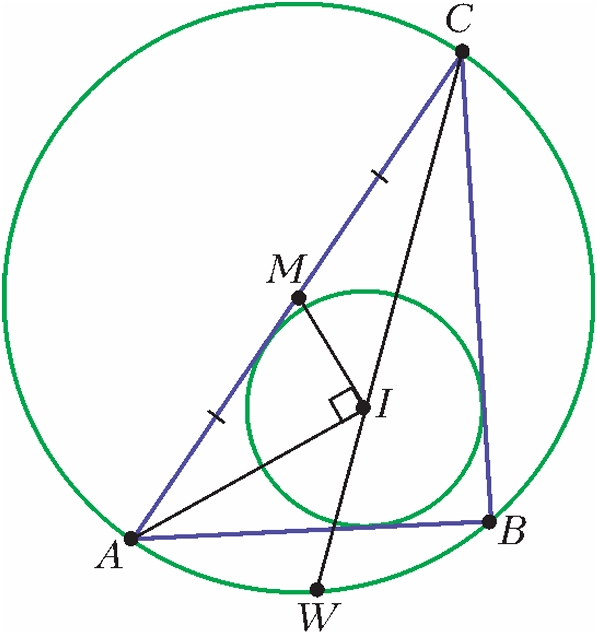
\includegraphics[width=0.65\linewidth]{pic.jpeg}
\end{center}

\textit{Рис. 2} \\
\noindent
\textcolor{Plum}{\textbf{M2480.}}
Для любых натуральных чисел \textit{m}
и \textit{n} докажите неравенства: \\
\noindent
\vspace{-1.5em}
\begin{align*}
    &a)\quad \frac{1}{2 \cdot \sqrt[m]{1}} + 
    \frac{1}{3 \cdot \sqrt[m]{2}} + 
    \dots +
    \frac{1}{(n + 1) \cdot \sqrt[m]{n}} < m; \\
    &b)\quad \frac{1}{1 \cdot \sqrt[m]{2}} + 
    \frac{1}{2 \cdot \sqrt[m]{3}} + 
    \dots +
    \frac{1}{n \cdot \sqrt[m]{n + 1}} < \frac{1}{\sqrt[m]{2} - 1}.
\end{align*}

\noindent
\textcolor{Plum}{\textbf{M2481*.}}
Дано натуральное число \textit{N} > 2. В
шеренгу выстроена команда из \textit{N}(\textit{N} + 1)
футболистов, среди которых нет двух
футболистов одинакового роста. Сэр Алекс
хочет удалить из шеренги \textit{N}(\textit{N} - 1) 
игроков так, чтобы остался ряд из 2\textit{N} игроков,
для которого выполнены следующие \textit{N}
условий: (1) никто не стоит между двумя
самыми высокими игроками, (2) никто не
стоит между третьим и четвертым по росту
\end{multicols}

\begin{tikzpicture}[remember picture, overlay]
    \node[anchor=south east, fill=Plum, minimum width=4.9em, minimum height=5.9em] at (current page.south east) {};
\end{tikzpicture}

\end{document}
